\chapter{Architecture and Design}
\label{chap:Architecture and Design}
% Apparently one needs to explain the architecture in this part. No mention of tools and co.

\begin{figure}
	\begin{center}
		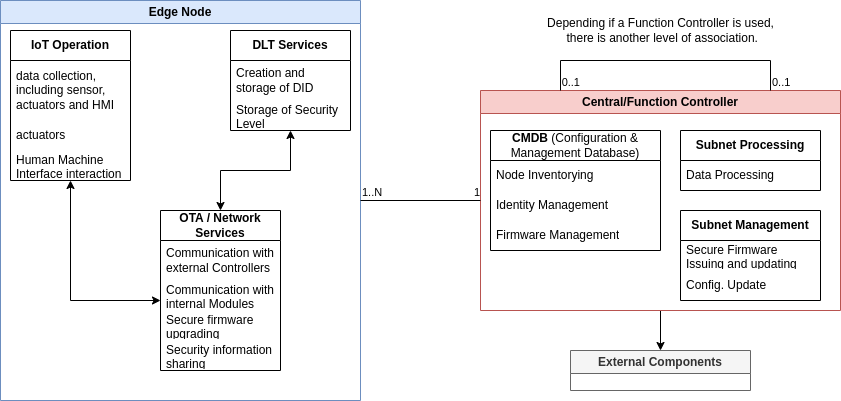
\includegraphics[width=0.95\textwidth]{figures/device-architecture-overview.png}
	\end{center}
	\caption{Device Architecture Overview}
	\label{fig:device-architecture-overview}
\end{figure}

\section{Actors} % (fold)
\label{sec:Actors-design}
In our architecture there will be a few actors, that play various roles, outlined in the below sections.

There will be a summarized device entity, that will be split up into two devices, as seen below in
Section~\ref{sec:Physical Components}, and further explained in Chapter~\ref{chap:Use Case Definition - Connected Cabin
	System}.
There will be a Manufacturer, that is responsible for the fabrication of said devices, as well as the creation of
Certificates and credentials, that will later be used by the devices and other entities for verification.
Further there shall be an auditor, that inspects said credentials and verifies them, or the necessary cases also
invalidation.
Finally an entity Infrastructure shall exist, that will enable the communication facilities for the entities.

We will assume a simplified and already predefined \textit{Authentication, Authorization and Accounting}, AAA, server
in order to simplify our environment.

Further external stakeholders include a certification authority and a vulnerability database.
% section Actors (end)

\section{Physical Components} % (fold)
\label{sec:Physical Components}

The composition of our physical architecture will entail two main devices of importance for us, as later defined in more
detail in Chapter \ref{chap:Use Case Definition - Connected Cabin System}, Section~\ref{sec:System Components}.

% The edge and controller nodes fulfill different responsibilities.

\subsection{Edge Nodes} % (fold)
\label{sec:Edge Nodes}
The edge nodes, also Internet of Things, IoT, nodes, are the frontier where direct interaction happens, be that sensing,
actuating or interaction through a Human Machine Interface, HMI.

Each edge node is uniquely identifiable through a Decentralized Identifier, DID, which will later be used for device
verification for outside entities through usage of a DLT. Furthermore, security levels, access levels will be stored on
each device. Through the use of MUDs, each device will be defined to have certain capabilities and access privileges,
which all will be enforced by the controller node.

\textbf{\textit{Warning:}} Whether we will store our DID in a Secure Element, SE, or on the SoC FLASH, is not yet decided.
% subsection Edge Nodes (end)

\subsection{Controller Nodes} % (fold)
\label{sub:Controller Nodes}
The controller nodes are managers of the edge nodes. They fulfill various responsibilities and shield edge nodes in a
subnet for increased security control
% subsection Controller Nodes (end)

% section Physical Components (end)

\section{Onboarding} % (fold)

\label{sec:Onboarding}
\begin{figure}
	\begin{center}
		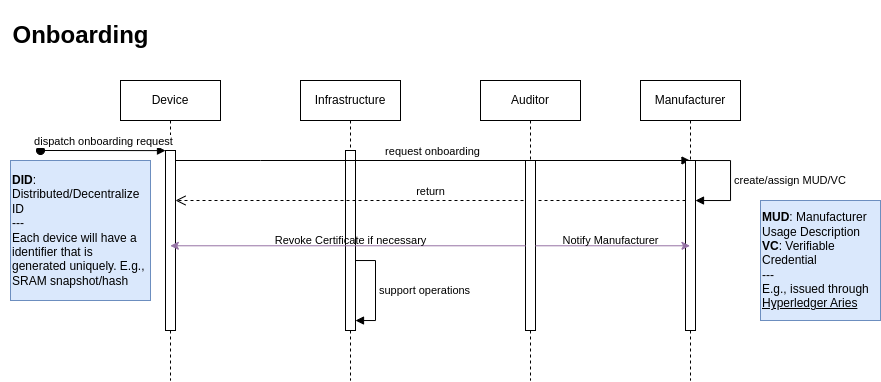
\includegraphics[width=0.95\textwidth]{figures/onboarding-sequence-diagram.png}
	\end{center}
	\caption{Onboarding Sequence Diagram}
	\label{fig:onboarding-sequence-diagram}
\end{figure}

The onboarding of a device can be observed in a sequence diagram in Figure~\ref{fig:onboarding-sequence-diagram}.
All of the actors in Section~\ref{sec:Actors-design} are involved.

We assume a device has been manufactured and that it is now at the desired location. In the first time setup, the device
will be either programmed to create a DID on setup, or will be assigned/created one in the manufacturing process,
depending on the computational and hardware facilities. Building up on that, as mentioned in
Section~\ref{sec:Physical Unclonable Function} the device will have unique key, but we will not be generating such a
function and neither derive a key for further use and we assume a predefined key to be placed into the device.

Both an edge and controller node shall have their DID, since
both will be managed and or inventoried by another instance or entity.
Necessary for this process is a valid MUD file, also issued by the manufacturer, on device fabrication or on first time
setup. This MUD does not necessarily need to be on the device, but an URL is needed, which points to the location of
such file, see Section~\ref{sec:Manufacture Usage Description}.
Each device shall request and onboarding by the manufacturer, which then verifies the DID, and in case of validity
issues a Verifiable Credential, VC, to the device.

In more detail, an edge node shall request onboarding from the controller node, which then forwards the request to the
manufacturer.

The Auditor then proceeds to verify the validity of the VC and checks for any known vulnerabilities, that might be
affect the device that requested the VC. The Auditor shall also monitor the VC periodically, in order to check for any
vulnerabilities the devices themselves might have missed. In case of an insecurity or vulnerability the auditor shall
notify both the device and the manufacturer and revoke the VC, until the device has been known to update its Firmware to
a secure version, see Section~\ref{sec:Secure Firmware Updating}.

\subsection{VC Verification} % (fold)
\label{sub:VC Verification}
The verification of a VC may happen through the usage of a Smart Contract. Therein the invalidation of
said smart contract happens through the fulfillment of the contract condition, which could be a discovered
vulnerability.
% subsection VC Verification (end)

% section Onboarding (end)


% NOTE: (aver) Emphasis 1
\section{Inventorying} % (fold)
\label{sec:Inventorying}

\begin{figure}
	\begin{center}
		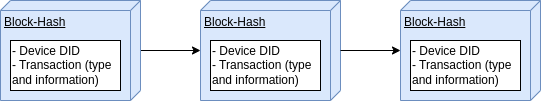
\includegraphics[width=0.95\textwidth]{figures/dlt-architecture.png}
	\end{center}
	\caption{DLT Architecture}
	\label{fig:dlt-architecture}
\end{figure}

Getting to the first emphasis of our thesis, we will explore, how we can safely and efficiently store and keep an
inventory of our devices.

For this we will rely on a DLT, in which any action will be saved as a block. The DLT used shall be permissioned and
possibly private, so that only those permissioned may be a part of this blockchain.
The DLT will work as a decentralized Configuration and Management Database, CMDB, as seen in
Figure~\ref{fig:dlt-architecture}. Transaction will be fulfilled by the controller node as indicated in
Figure~\ref{fig:device-architecture-overview}.

% section Inventorying (end)


\section{Operations} % (fold)
\label{sec:Operations}

In order to be able to simulate the whole device lifecycle, we will also implement simple day-2-day operations, such as
reading out sensors, actuating or minor interactions through HMIs.

Depending on the device type, edge or controller, further responsibilities are expected. A controller node has to
constantly check against the DLT, whether there were any new vulnerabilities discovered and if the VC was consequently
revoked, as mentioned before, the controller node has to check its own status, as well as the ones of the subnet of
edge nodes. If such were the cases, concerned devices need be recertified.

% TODO: (aver) possibly extend with real-time local security monitoring

% section Operations (end)


% NOTE: (aver) Emphasis 2
\section{Secure Firmware Updating} % (fold)
\label{sec:Secure Firmware Updating}

As the second emphasis of this thesis we aim to provide a secure update mechanism for outdated and or vulnerable
firmware versions.

\begin{figure}
	\begin{center}
		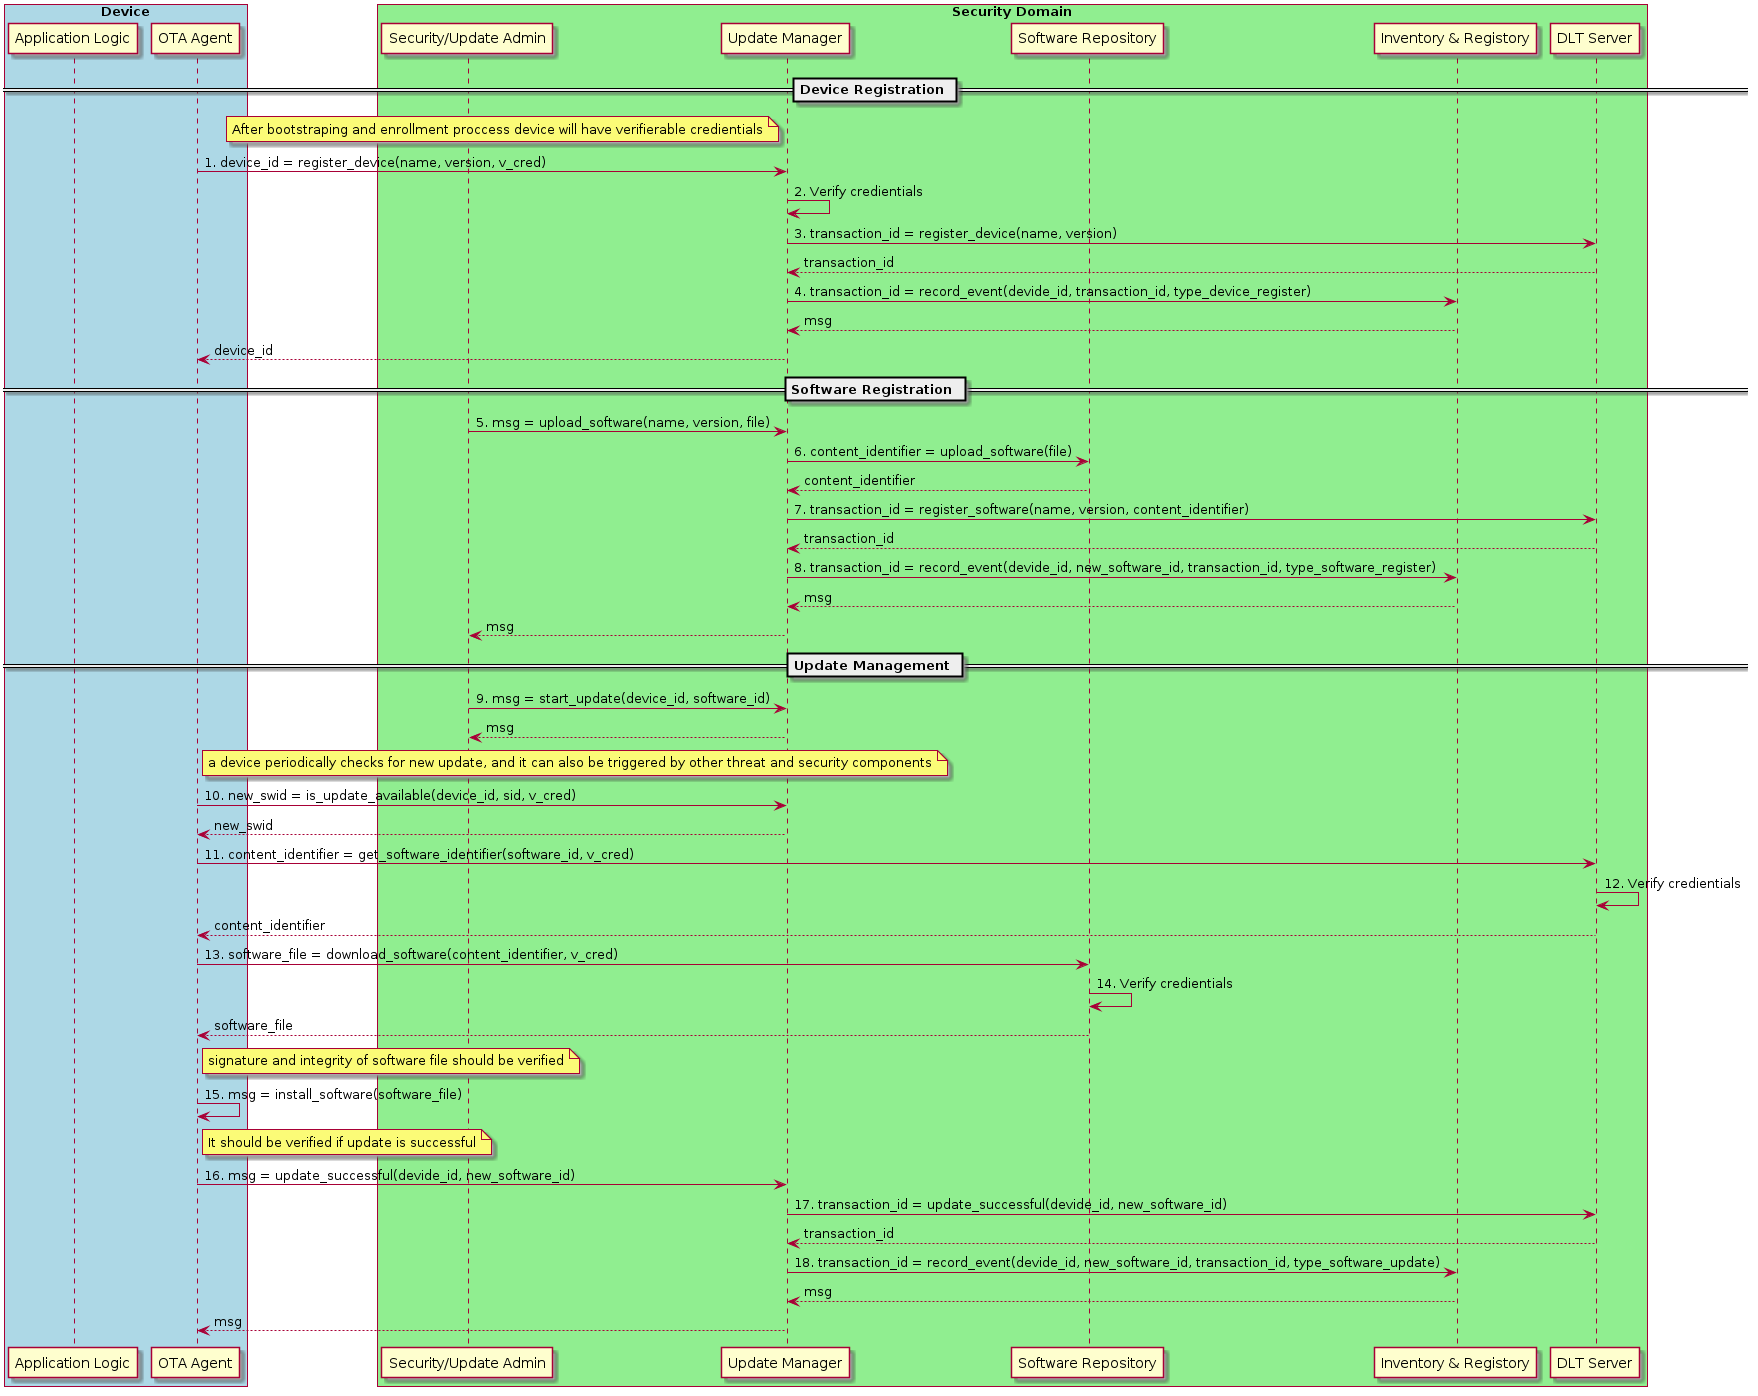
\includegraphics[width=0.95\textwidth]{figures/ota-update-certify-V1.2.png}
	\end{center}
	\caption{CERTIFY OTA Update \cite{certifyproject2023}}
	\label{fig:ota-update-certify}
\end{figure}

% TODO: (aver) research and explain possible update mechanisms.
% 2023-07-04: Also wait for Eryk to send me documents on existing mechanisms.

% section Secure Firmware Updating (end)

\section{Secure Information Sharing} % (fold)
\label{sec:Secure Information Sharing}

In order to enable the sharing of information related to the security of the device, we will rely on directional
information sharing, meaning, the devies receive vulnerability information, updates and MUD files, while external
sources receive status updates and co. of the devices concerned.

These information can be embedded into transaction inside the DLT, depending on the importance of the information, it
can also be shared through less sophisticated measures.

% section Secure Information-Sharing (end)
